\section{EXPERIMENTAL RESULTS} \label{experiments}

The experiments in this work focus on comparing the performance of a DDPG and PPO agent trained to select actions using compressed states from a World Model network to the performance of the baseline implementation of DDPG and PPO trained using the convolutional component to process raw state images. In order to evaluate the performance of the World Model for deep reinforcement learning over the current evolutionary method, we also require a baseline for the simple controller trained with CMA-ES. We will evaluate the effectiveness of the World Model trained only on 10000 random rollouts of the environment as done in \cite{1.0.0}, then retrained on 1000 random and 1000 policy rollouts using the previous iteration's trained controller network. The list of experiments is as follows:

\begin{enumerate}
	\item Train a baseline controller with an untrained VAE and MDRNN using the CMA-ES strategy.
	\item Sample 10000 rollouts using a random (Brownian noise) agent, then train the first iteration of VAE and MDRNN on experience sequences from these rollouts. Then train the first iteration controller with CMA-ES using the first iteration World Model.
	\item Sample 1000 rollouts using a random (Brownian noise) agent and 1000 rollouts using the first iteration controller, then train the second iteration of VAE and MDRNN on experience sequences from these 2000 rollouts. Then train the second iteration controller with CMA-ES using the second iteration World Model.
	\item Train a baseline DDPG and PPO agent with stacked grayscale images of dimension 64x64x2 as input to the convolutional component.
	\item Train the DDPG and PPO with the compressed state vector of size 288 from the first iteration World Model as input to the single-layer before the feed-forward component.
	\item Train the DDPG and PPO with the compressed state vector of size 288 from the second iteration World Model as input to the single-layer before the feed-forward component.
\end{enumerate}

\subsection{Results}

The above experiments were run on a 3.6GHz 8-core Linux desktop with 64GB RAM and a NVIDIA RTX 2070 GPU with 8GB memory. Figure~\ref{fig:wm} below shows the best score (thin line) and rolling 100-generation average (thick line) of the population at each of the 250 generations of CMA-ES parameter evolution for training the first and second iteration controller. The green line represents the baseline from experiment 1, the blue lines represent the best and average score for the first iteration controller from experiment 2 and the red lines represent the best and average score for the second iteration controller from experiment 3. The first iteration controller achieved a maximum average of 681 and a maximum best score of 796 while the second iteration controller achieved a maximum average of 885 and a maximum best score of 909.

\begin{figure}[!ht]
	\begin{subfigure}{}
		\centering
		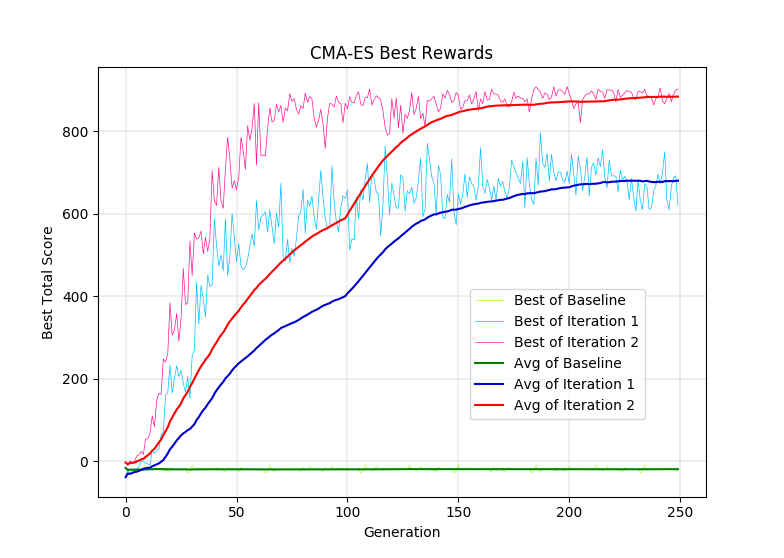
\includegraphics[width=0.50\textwidth]{images/WM4.png}\caption{Best Population Scores for CMA-ES with World Models}\label{fig:wm}
	\end{subfigure}
	\begin{subfigure}{}
		\centering
		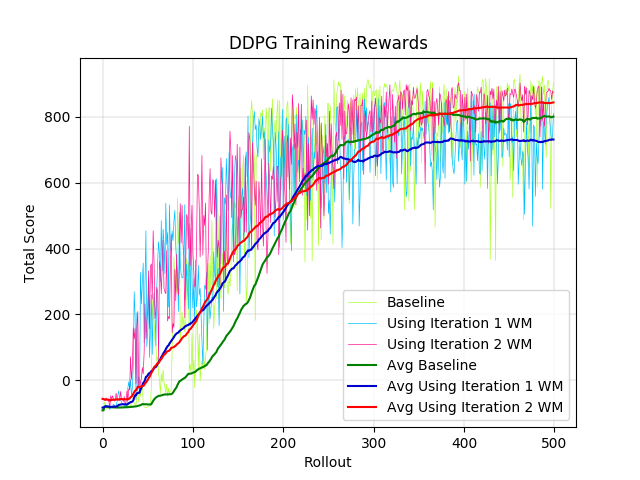
\includegraphics[width=0.50\textwidth]{images/DDPG3.png}\caption{DDPG Training Scores (left) and PPO Training Scores (right)}\label{fig:rl1} 
	\end{subfigure}
	\begin{subfigure}{}
		\centering
		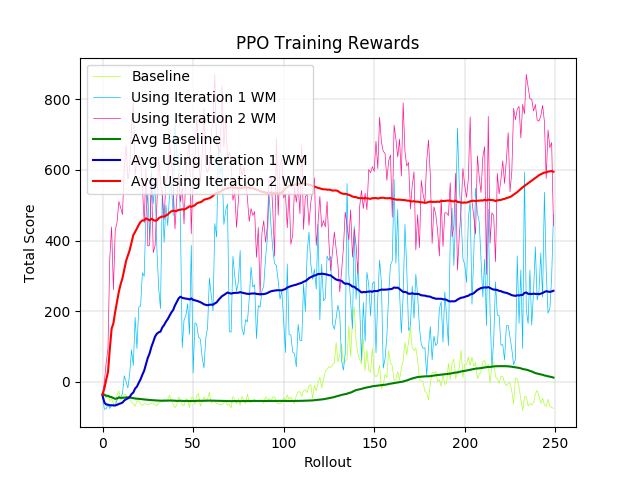
\includegraphics[width=0.50\textwidth]{images/PPO3.png}\caption{DDPG Training Scores (left) and PPO Training Scores (right)}\label{fig:rl2} 
	\end{subfigure}
\end{figure}

Figure \ref{fig:rl1} below shows the training scores (thin line) and rolling 100-rollout average (thick line) of the DDPG agents trained for 500 rollouts (left) and PPO agents trained for 250 rollouts (right). In each graph, the green lines represent the baseline from experiment 4, the blue lines represent training the agent using the first iteration World Model from experiment 5 and the red lines represent training the agent using the second iteration World Model from experiment 6. For the baseline, the DDPG agent achieved a maximum score of 929 and maximum average of 816 and the PPO agent achieved a maximum score of 212 and maximum average of 45. Using the first iteration World Model, the DDPG agent achieved a maximum score of 890 and maximum average of 734 and the PPO agent achieved a maximum score of 734 and maximum average of 306. Using the second iteration World Model, the DDPG agent achieved a maximum score of 904 and maximum average of 844 and the PPO agent achieved a maximum score of 871 and maximum average of 597.

Following the training of all agents for the baseline and both iterations of World Model, the model of each agent was saved at the point in training where it had achieved the highest score over 10 test rollouts. Then, for each saved model, the agent was evaluated over 100 consecutive trials providing a mean score and standard deviation. Table \ref{tab:trials} below shows the mean ($\pm$ standard deviation) of each agent over the baseline, and using each iteration of World Model. The best average trial score for each agent is highlighted in bold.

\begin{table}[h]
    \caption{Average 100-trial Scores Across Agents}\label{tab:trials}
 	\hspace{2em}
	\centering % center the table
	\small % text size of table content
	\begin{tabular}{cccc} % alignment of each column data
    \toprule[\heavyrulewidth]\toprule[\heavyrulewidth]
    \textbf{\ \ Agent\ \ } 	& \textbf{Baseline} & \textbf{World Model 1} 	& \textbf{World Model 2} 	\\
    \midrule
    CMA-ES			& -46 $\pm$ 13				& 632 $\pm$ 184						& \textbf{825 $\pm$ 150}	\\
 	\midrule
    DDPG			& \textbf{845 $\pm$ 167}	& 710 $\pm$ 206						& 842 $\pm$ 78				\\
 	\midrule
    PPO				& 153 $\pm$ 137	 			& 739 $\pm$ 186						& \textbf{812 $\pm$ 158}	\\
    \bottomrule[\heavyrulewidth] 
    \end{tabular}
\end{table}

\subsection{Discussion}

There is a clear difference between the relative performance of benchmarks for each agent algorithm and the best scoring trial for that agent. Considering the baseline, we found that a simple controller trained with the CMA-ES strategy using an untrained VAE and MDRNN was effectively a random agent that simply moved forward along the initial track. Comparing the first and second iteration of training the controller with a World Model, the improvement in average 100-trial score from 632 to 825 indicated that training on policy sampled rollouts was necessary to accurately represent reward bearing states. Furthermore, the second iteration was only trained on 2000 total rollouts compared to the 10000 total rollouts in the original paper \cite{1.0.0}. While our simplified implementation for training the controller with a population size of 16 instead of 64 didn't achieve an average above 900, this may still provide a contrast in the performance variation over different training configurations.

For the DDPG agent, the baseline was able to achieve the highest 100-trial average score of 845, however when compared to the second-best performing trial averaging 842 using the second iteration World Model, we observe the score standard deviation when using the World Model is less than half of that of the baseline. This is also seen in Figure \ref{fig:rl1} where the variation in scores at each rollout is reduced using the World Model. Considering both iterations of the World Model for training the DDPG agent, Figure \ref{fig:rl1} also shows faster and more stable improvement in scores. Therefore, with a smaller state representation given by the World Model, this allows the agent to more quickly learn a mapping from the relevant state information to an optimal action. However, as the baseline was also able to control the training of the convolutional component representing the encoder of a World Model VAE, where the VAE in the World Model was fixed after initial training, this could suggest that an independently trained World Model may not encode the most relevant features for the action selection task. For future work, this could be addressed by using the policy gradients from training an agent in the environment to further optimize a pre-trained World Model for the particular task.

As PPO involves more stochastic parameter optimization, there is a large fluctuation in the training scores observed. We therefore evaluated the PPO agent using the saved parameters at the rollout that achieved the highest training score. For the baseline, the agent was unable to learn a stable policy and eventually diverges back to a random policy. This could be due to the large number of parameters from the convolutional component that needs to process the high dimensional image state input. In contrast, when using the World Model, Figure \ref{fig:rl2} shows the PPO agent was able to learn a policy within 50 episodes that was able to achieve a maximum training score of 734 and 871 using the first and second iteration World Models respectively. Therefore, the World Model has potential to significantly improve the effectiveness and efficiency of the PPO algorithm for learning complex tasks from high dimensional image states.

It can be observed in Table \ref{tab:trials} that all agents using the second iteration World Model were able to achieve an average score within the 800s over 100 consecutive trials, being the highest scoring trials for that agent, except in the case of the DDPG agent which scored 3 points below its baseline. While these average scores are within 10\% of the minimum threshold of 900 for solving the environment, it is important to consider the implications of this requirement. With the maximum cumulative reward of 1000 from reaching every tile, the agent also experiences a maximum cumulative negative reward of -100 (-0.1 over 1000 time steps). Therefore, in order to score above 900, the agent needs to visit every tile in a single round of the circuit due to the time limit. Ha and Schmidhuber reported in the original paper that the simple controller trained with the CMA-ES strategy was able to achieve an average of 906 $\pm$ 21, which suggests that the agent prioritized visiting every tile in the 1000 time step limit. In the case of DDPG, it was found that the learned policy would reach a local optimum where the agent would prioritize the greedy action of speeding up in order to complete the track faster. However, this would then cause the agent to cut sharp turns and miss a tile, where it was then unable to reach the missed tile in a second round of the circuit in the given time limit. In rollouts where the agent slowed down to navigate turns, it was then able to complete the track. In other cases, a small mistake would cause the car to spin, where if the agent was able to regain control, it would proceed in the opposite direction where the tiles had already been reached. In the case of PPO, since this algorithm is stochastic in nature, this increases the chance of taking a suboptimal action. These examples emphasize the challenge of the car racing environment for reinforcement learning agents, where approximating the value of each state in a rollout can lead to learning a greedy suboptimal policy. Ha and Schmidhuber refer to this as the credit assignment problem, which motivated the use of evolutionary algorithms which optimize a policy based on the total reward from a rollout. Addressing this problem in deep reinforcement learning would be an interesting area for future work.

\subsection{Future Work}

The reinforcement learning agents trained using the World Model were close to solving the \texttt{CarRacing-v0} environment. A simplified training process with 16 parallel agents was used due to time constraints, however, with more fine-tuning of hyperparameters, it may be possible to establish achieve a new state of the art in reinforcement learning algorithms for solving \texttt{CarRacing-v0} which have not been able to achieve an average 100-trial score of more than 600 without discretizing the action space \cite{3.0, 3.1, 3.2}.

In another area of future work, the pre-trained World Model can be further optimized during policy optimization, enabling the agent to fine-tune the features encoded in the latent space that are most important for action selection, such as identifying which tiles have not been visited. Ha and Schmidhuber also suggested incorporating attention mechanisms into the MDRNN to focus on important temporal events and their consequences on future states. A recent paper incorporated visual attention within the VAE and MDRNN for a controller trained with the CMA-ES strategy \cite{1.1}. This could be adapted for a deep reinforcement learning agent to train the VAE and MDRNN during policy optimization.